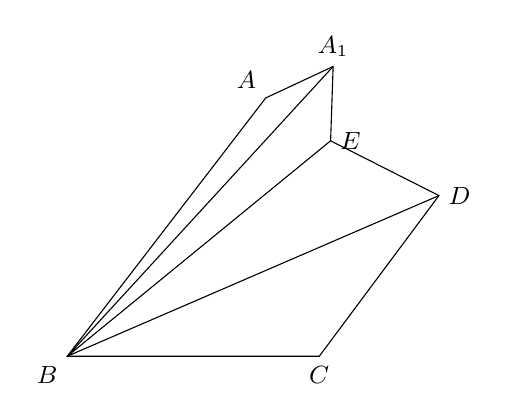
\begin{tikzpicture}[scale=.8, every node/.style={font=\small}]
  \coordinate (B) at (0,0);
  \coordinate (C) at (4.0,0);
  \coordinate (D) at (5.9,2.55);
  \coordinate (E) at (4.18,3.42);
  \coordinate (A1) at (4.22,4.6);
  \coordinate (A) at (3.15,4.1);
  \draw (B)--(C)--(D)--(E)--(A1)--(A)--cycle;
  \draw (B)--(E) (B)--(D) (B)--(A1);
  \node[below left] at (B) {$B$};
  \node[below] at (C) {$C$};
  \node[right] at (D) {$D$};
  \node[right] at (E) {$E$};
  \node[above] at (A1) {$A_1$};
  \node[above left] at (A) {$A$};
\end{tikzpicture}
